\documentclass[aspectratio=169]{beamer}
\usetheme{Madrid}
\usepackage{comment}
\usepackage{ragged2e}
\usepackage{amsmath}
\usepackage{xcolor}
\usepackage{multirow}
\usepackage{multicol}
\usepackage{caption}
\usepackage{tikz}
\usetikzlibrary{shapes.multipart}
\usetikzlibrary{calc}
\usetikzlibrary{shapes, arrows, positioning}
\usetikzlibrary{decorations.pathreplacing}
\usetikzlibrary{patterns}
\usepackage{booktabs}
\usepackage[title]{appendix}
\usepackage{booktabs}
\usepackage{appendixnumberbeamer}
\setbeamertemplate{caption}[numbered]
\usepackage{hyperref}
\hypersetup{
	colorlinks=false,
	linkcolor=blue,
	filecolor=blue,      
	urlcolor=blue,
}
\usepackage{graphicx}
\usepackage{mathtools}
\usepackage{amssymb}
\usepackage{amsthm}
\usepackage{thmtools}
\usepackage{natbib}
\newtagform{nonums}[\phantom]{}{}
\usetagform{nonums}

\newcommand\scalemath[2]{\scalebox{#1}{\mbox{\ensuremath{\displaystyle #2}}}}

\def\boxit#1{%
	\smash{\color{red}\fboxrule=1pt\relax\fboxsep=2pt\relax%
		\llap{\rlap{\fbox{\vphantom{0}\makebox[#1]{}}}~}}\ignorespaces
}
\renewcommand{\today}{\ifcase \month \or January\or February\or March\or %
	April\or May \or June\or July\or August\or September\or October\or November\or %
	December\fi, \number \year} 





% \AtBeginSection[]
% {
% 	\begin{frame}[noframenumbering,]{Table of Contents}
% 		\scriptsize
		
% 			\tableofcontents[hideallsubsections,hideothersubsections,currentsection]

		
% 	\end{frame}
% }	
\usepackage{pifont}
\usepackage{tikz}

\definecolor{cec1d24}{RGB}{236,29,36}
\definecolor{cffffff}{RGB}{255,255,255}

\newcommand{\cmark}{\ding{51}}
\newcommand{\ucmark}{\tikz[y=0.80pt,x=0.80pt,yscale=-0.02,xscale=0.02, inner sep=0pt, outer sep=0pt]%
  {\path[fill=cec1d24,nonzero rule] (635.8833,600.0000) .. controls
    (651.0771,599.6647) and (665.7558,591.6224) .. (673.9783,577.5525) .. controls
    (682.1001,563.3625) and (681.7384,546.6500) .. (674.5074,533.1862) --
    (378.4699,21.6487) .. controls (370.6590,8.7662) and (356.3424,0.0975) ..
    (340.1099,-0.0063) .. controls (323.6499,0.0972) and (309.3362,8.7657) ..
    (301.4862,21.6487) -- (5.4612,533.1862) .. controls (-1.7257,546.6500) and
    (-2.0877,563.3625) .. (5.9903,577.5525) .. controls (14.2570,591.6225) and
    (28.9353,599.6650) .. (44.0853,600.0000) -- (635.8853,600.0000);
    \path[fill=cffffff,nonzero rule] (340.1208,75.7875) -- (71.0683,540.8450) --
    (608.8933,540.8450) -- (340.1058,75.7950);
    \path[fill=black,nonzero rule] (303.5900,225.7800) .. controls
    (280.4500,225.7300) and (276.9200,248.1400) .. (276.8800,250.6200) .. controls
    (276.9200,262.4400) and (285.4000,277.1700) .. (309.1600,279.4100) .. controls
    (309.1600,279.4100) and (313.7700,280.0900) .. (313.6600,283.0900) .. controls
    (313.7700,285.9400) and (313.7800,284.9700) .. (312.3400,286.5300) .. controls
    (310.8500,288.2300) and (298.5500,299.6400) .. (298.3100,302.6600) .. controls
    (296.9800,316.8800) and (300.1800,335.2800) .. (303.0900,345.9400) .. controls
    (303.0900,345.9400) and (306.6000,354.7800) .. (303.8800,361.0000) .. controls
    (301.0600,367.4700) and (289.0000,397.7400) .. (288.0000,399.5600) .. controls
    (285.1300,404.8200) and (284.0000,409.1400) .. (285.8800,415.4100) .. controls
    (284.6600,416.1100) and (264.4700,428.8800) .. (264.4700,428.8800) .. controls
    (264.4700,428.8800) and (261.3500,421.5100) .. (253.5900,419.3800) .. controls
    (245.7000,417.1100) and (239.1800,418.1800) .. (232.7200,405.9100) --
    (226.8800,396.4100) .. controls (226.8800,396.4100) and (225.6700,392.9300) ..
    (219.7500,391.6200) .. controls (213.9300,390.4900) and (206.1000,388.3000) ..
    (202.8100,388.4700) .. controls (198.6100,388.8800) and (195.2200,387.7300) ..
    (189.5900,394.2800) .. controls (185.0800,399.5300) and (112.8800,524.4700) ..
    (112.8800,524.4700) -- (286.4100,524.4700) .. controls (286.4100,524.4700) and
    (290.7100,524.0000) .. (289.5900,519.9700) .. controls (288.2700,516.1900) and
    (267.3800,441.8100) .. (267.3800,441.8100) -- (291.4400,426.7500) .. controls
    (291.4400,426.7500) and (293.3600,429.9900) .. (300.4400,426.7500) .. controls
    (307.3800,423.4800) and (309.9700,421.7500) .. (309.9700,421.7500) .. controls
    (309.9700,421.7500) and (313.9200,421.4900) .. (313.4100,413.0300) .. controls
    (316.1700,411.3100) and (341.9700,395.0600) .. (341.9700,395.0600) .. controls
    (341.9700,395.0600) and (332.8400,417.6000) .. (331.9100,427.5600) .. controls
    (331.2100,437.4600) and (327.6900,504.1200) .. (327.6900,504.1200) .. controls
    (327.6900,504.1200) and (328.1300,509.2200) .. (324.7800,510.2200) .. controls
    (321.2800,511.1700) and (305.7200,515.5000) .. (305.7200,515.5000) .. controls
    (305.7200,515.5000) and (301.3900,516.2100) .. (301.5000,519.7200) .. controls
    (301.3900,523.0400) and (303.0200,524.3400) .. (304.9400,524.4700) .. controls
    (306.9300,524.3400) and (355.7200,524.4700) .. (355.7200,524.4700) .. controls
    (355.7200,524.4700) and (360.7100,525.0000) .. (361.5300,518.4100) .. controls
    (362.3400,511.9900) and (371.5900,445.5000) .. (371.5900,445.5000) .. controls
    (371.5900,445.5000) and (367.5700,444.4500) .. (367.6200,440.5000) .. controls
    (367.5700,436.3200) and (367.5600,433.2000) .. (368.9400,431.5000) .. controls
    (370.1600,429.9500) and (384.8300,413.0400) .. (394.8800,389.5300) .. controls
    (396.4200,386.0300) and (397.5600,389.1300) .. (397.7800,390.0600) .. controls
    (398.2100,390.7500) and (417.2800,442.6600) .. (419.4700,444.7200) .. controls
    (421.8400,446.5600) and (473.3600,488.2300) .. (474.5000,489.0900) .. controls
    (475.6400,489.8600) and (478.9100,492.1100) .. (479.0000,499.3800) .. controls
    (478.9100,506.7600) and (475.9700,512.6300) .. (473.9700,514.9700) .. controls
    (472.0500,517.1900) and (468.8000,520.4500) .. (468.6900,521.8400) .. controls
    (468.8000,523.3800) and (470.2800,524.3400) .. (471.3400,524.4700) .. controls
    (472.5600,524.3400) and (479.2500,524.3400) .. (479.8100,524.4700) .. controls
    (480.5500,524.3400) and (489.3400,525.0100) .. (495.4100,514.1900) .. controls
    (501.7300,503.5300) and (513.1200,484.3400) .. (513.1200,484.3400) .. controls
    (513.1200,484.3400) and (515.5800,480.5600) .. (512.0600,478.2500) .. controls
    (508.4000,476.0100) and (502.7100,474.7100) .. (499.3800,471.1200) .. controls
    (495.8600,467.5500) and (462.9400,429.6400) .. (462.3400,428.8800) .. controls
    (461.9600,428.3400) and (457.7100,423.7600) .. (452.2800,426.2200) .. controls
    (450.7000,424.0900) and (448.8400,421.2200) .. (448.8400,421.2200) .. controls
    (448.8400,421.2200) and (439.4600,364.4600) .. (429.5300,340.4100) .. controls
    (431.8000,339.0000) and (434.8100,336.7200) .. (434.8100,336.7200) .. controls
    (434.8100,336.7200) and (442.7200,343.5500) .. (449.3800,336.4400) .. controls
    (456.0900,329.2300) and (455.6000,329.4100) .. (454.4100,326.1600) .. controls
    (453.3200,322.9000) and (452.8300,321.9100) .. (450.4400,320.5900) .. controls
    (448.2700,319.3000) and (444.5200,315.5500) .. (444.6200,308.9700) .. controls
    (444.5200,302.5400) and (441.7400,284.8000) .. (438.5300,277.2800) .. controls
    (435.5500,269.8300) and (434.5600,261.5500) .. (422.9100,256.4400) .. controls
    (404.4800,248.2100) and (379.8000,243.3100) .. (361.8100,247.9700) .. controls
    (356.8300,249.3000) and (340.8200,261.0500) .. (339.3100,261.9700) .. controls
    (337.8900,262.6800) and (331.6400,265.2600) .. (332.1900,259.8400) .. controls
    (333.4500,247.4700) and (322.7500,225.7300) .. (303.5900,225.7800) --
    cycle(394.8800,275.9700) .. controls (394.8800,275.9700) and
    (408.4700,275.8400) .. (411.5300,276.2200) .. controls (414.3400,276.5000) and
    (416.0300,280.1900) .. (416.0300,280.1900) -- (429.0000,325.8800) --
    (424.2500,328.7800) .. controls (421.5800,323.2700) and (397.9000,287.2600) ..
    (393.0300,280.4700) .. controls (389.9100,276.1000) and (394.8800,275.9700) ..
    (394.8800,275.9700) -- cycle(331.0000,332.8100) .. controls
    (331.5700,332.7900) and (332.2200,332.9700) .. (332.7200,333.2800) .. controls
    (337.8300,336.2000) and (347.5100,344.5400) .. (355.7200,356.0000) .. controls
    (356.7000,357.3200) and (355.7200,361.2800) .. (355.7200,361.2800) --
    (348.5900,376.0600) .. controls (348.5900,376.0600) and (317.8500,395.3700) ..
    (315.5000,396.9100) .. controls (312.9600,398.3000) and (311.5500,396.9300) ..
    (313.9400,393.7500) .. controls (327.6400,375.1200) and (332.7200,353.0000) ..
    (329.5300,335.1200) .. controls (329.2600,333.4800) and (330.0500,332.8500) ..
    (331.0000,332.8100) -- cycle;}}

\pagenumbering{gobble}

% \setbeamercovered{transparent}
\title{Resource Reallocation with Carbon Emission Policies}
\author{Seyyed Morteza Aghajanzadeh}
\date{\today}
\subtitle{}
\institute[SSE]{Stockholm School of Economics}
 
\begin{document}
\maketitle
\section{Motivation}
\begin{frame}{Motivation}\large 
	\begin{itemize}
        \item Climate crisis intensifies: rising temperatures, extreme weather.
        \pause
        \item Government interventions steer markets towards sustainability.
        \item Key policies: carbon pricing, renewable subsidies to curb emissions.
        \item Economic impacts:
            \begin{itemize}
                \item[$\blacksquare$] Limitation in fossil fuel usage.
                \item[$\blacksquare$] Adoption of renewable technologies.\pause
                \item[$\blacksquare$] {\bf Reallocation of resources to greener firms/industries.}
            \end{itemize}
	\end{itemize}
\end{frame}
\begin{frame}{Research Question}
	\begin{itemize}
		\item \textbf{What is the Economic Outcomes of environmental policies due to \underline{resources reallocation}?}
		\begin{itemize}
			\item Industry output
			\item Firm-level productivity
			\item Sector size
			\item Emission intensity
			\item Total Emission
		\end{itemize}
	\end{itemize}
\end{frame}


\begin{frame}{Literature and Contribution}
	\begin{itemize}
		\item Effectiveness of Carbon policies:
		\begin{itemize}
			\item \cite{martinsson2024effect,shapiro2018pollution,ahmadi2022carbon,andersson2019carbon} \\ Contribution: \textbf{Quantify substitution between green and brown capital}
		\end{itemize}
		\pause
		\item Misallocation:
		\begin{itemize}
			\item 	\cite{whited2021misallocation,hsieh2009misallocation,ai2020financial,asker2014dynamic}\\
			Contribution: \textbf{Misallocation (Reallocation) in the context of environmental policies}
		\end{itemize}
		\pause
		\item Climate Policy Design:
		\begin{itemize}
			\item \cite{acemoglu2012competing,acemoglu2016transition,oehmke2023theory}\\
			Contribution: \textbf{Assess alternative instruments in Emission Intensity / resource reallocation trade off}
		\end{itemize}
	\end{itemize}
	
\end{frame}

\begin{frame}{Road map}
	\begin{enumerate}
		\item Develop Economic model with Emission  \only<2->{\cmark}
		\item Characterize the allocation of resources  \only<2->{\cmark}
		% \item {Provide a definition of Green and Brown capital} \only<3->{\ucmark}
		\item Estimate the model by Swedish data \only<3->{\ucmark}
		\item Compare the optimal Policy with resource reallocation \only<3->{\ucmark}
		\item Discuss the cost of the environmental policies \only<3->{\ucmark}
	\end{enumerate}
\end{frame}


\section{Model}

\begin{frame}{Standard Framework}{\cite{hsieh2009misallocation}}
	\begin{itemize}
		\item Heterogeneous monopolistic competitive firms
		\item Partial equilibrium
		\item Cobb-Douglas Production function 
		\item CES aggregator for output
		% \begin{equation}
    Y_s = \left(
        \sum_{i=1}^I Y_{si}^{\frac{\sigma_s-1}{\sigma_s}}
    \right)^{\frac{\sigma_s}{\sigma_s-1}}
\end{equation} \hfill
		% \begin{equation}
    Y = \Pi_1^S Y_s^{\lambda_s}, \quad \text{where} \quad \sum^S \lambda_s = 1
\end{equation}
		\item Normal aggregation of emissions
		% \begin{equation}\label{eq:sector_emission}
    E_s = \sum_{i=1}^I E_{si}, \quad E = \sum_{s=1}^S E_s
\end{equation}
	\end{itemize}

\end{frame}



\begin{frame}{Extension}{Production functions}\label{Production_Functions}
	\begin{itemize}
		\item Industry $s$, firm $i$:
	\end{itemize}
	\begin{equation}
		Y_{si} = {\only<1>{\textcolor{blue}}{\hat{A}_{si}}\textcolor{red}{\hat{K}_{si}}^{\beta_s} L_{si}^{1-\beta_s}} \only<2->{\quad,\qquad \textcolor{red}{\hat{K} = (
			\alpha_s G_{si}^{\frac{\gamma_s-1}{\gamma_s}} + (1-\alpha_s) B_{si}^{\frac{\gamma_s-1}{\gamma_s}}
		) ^ {\frac{\gamma_s}{\gamma_s-1}}}}
	\end{equation}
	\\
	\uncover<2->{\begin{equation}
		E_{si} = \textcolor{blue}{\tilde{A}_{si}} B_{si}
	\end{equation}
	\hfill
	\hyperlink{Emission_General_Model}{\beamerbutton{Emission General Model}}}
	\begin{itemize}\footnotesize
		\item $\hat{A}_{si}$: total factor of productivity
		\uncover<2->{\item $\alpha_s$: importance of Green capital in the production
		\item $\gamma_s$: elasticity of substitution between Green and Brown capital
		\item $\tilde{A}_{si}$: emission inefficiency
		\item Firms maximize over G, B, and L }
	\end{itemize}
	\hfill
	\hyperlink{Firm_profit}{\beamerbutton{Firm's profit}}
\end{frame}


\begin{frame}{Estimation }
	\begin{table}[http]
		\resizebox{0.3\textwidth}{!}{\input{Tables/Panel A}}
	\end{table}
	
\end{frame}

\begin{frame}{Calibration}\label{estimation_result}
	\begin{itemize}\footnotesize
		% \item My goal is to estimate the parameters sector by sector for Sweden
		\item I just reasonably calibrate the model to match the summary statistics of \cite{martinsson2024effect}
		% \item I will set the $\hat{A} =$  \input{values/A hat estimate} to match the total output in the economy ($\sim 10$ BSEK).
	\end{itemize}
	% \begin{table}[http]
	% 	\resizebox{0.3\textwidth}{!}{\input{Tables/Panel A}}
	% \end{table}
	\begin{table}[ht]
		\centering
		\resizebox*{0.4\textwidth}{!}{\begin{tabular}{@{}ccc@{}}
		\toprule
		\textbf{Parameter} & \textbf{Value} & \textbf{Source/Moment}\\
		\midrule 
		\multicolumn{3}{c}{Panel A: Estimated Value} \\
		\midrule
		$\gamma$ & \input{values/gamma estimate} & $\Delta(\frac{E}{PY})/\Delta(\frac{C}{PY})$ \\
		$\tilde{A}$ & \input{values/A tilde estimate} & $ E/PY $\\ 
		\midrule
		\multicolumn{3}{c}{Panel B: Inputs} \\
		\midrule
		$\sigma$ & $5$ & - \\
		$r$ & $5\%$ & - \\
		$w$ & $500$ TSEK & - \\
		\midrule 
		\multicolumn{3}{c}{Panel C: Calibrated Value} \\
		\midrule
		$\beta_s$ & $0.6$ &  \cite{martinsson2024effect}\\
		$\alpha_s$ & \input{values/alpha estimate} & {$G/B$}, \cite{wiedemann2023green} \\
		\bottomrule
		\end{tabular}}
	\end{table}
		{
		\hfill
		\hyperlink{sensitivity}{\beamerbutton{Sensitivity of $\alpha$}}}
\end{frame}





\section{Results}



\begin{frame}{Emission and Production}{Results}\label{emission_production}

	{\begin{figure}[http]
		\centering
		\only<1>{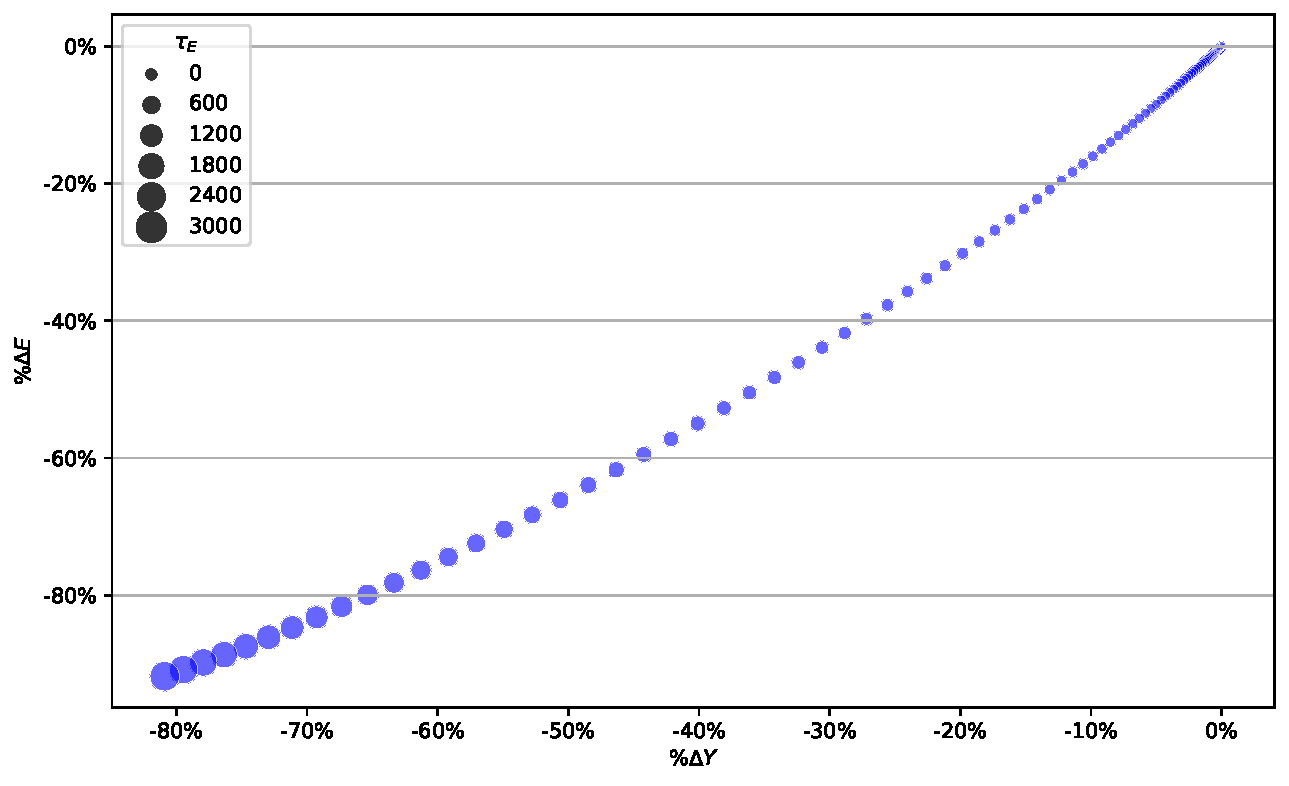
\includegraphics[width=.6\textwidth]{Figures/emission_production_1.pdf}}
		\only<2>{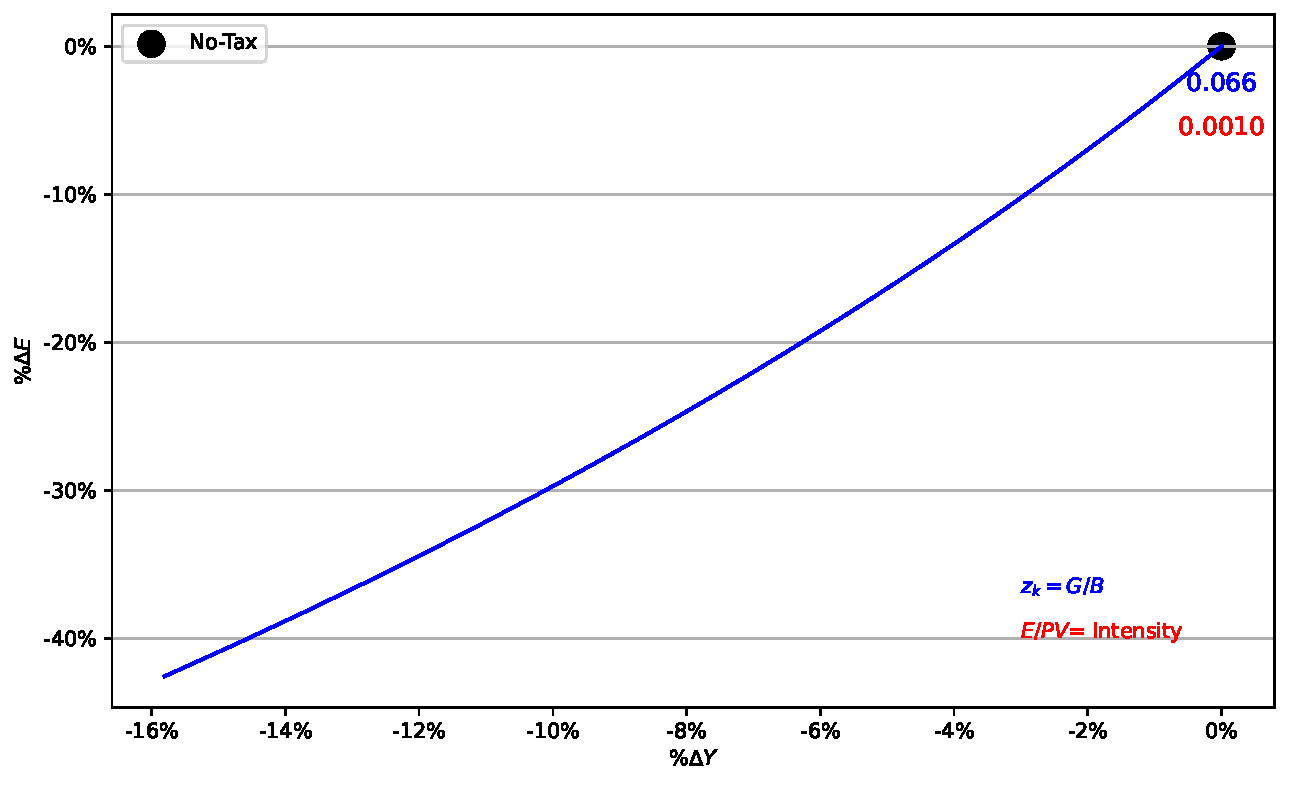
\includegraphics[width=.6\textwidth]{Figures/emission_production_2_1.pdf}}
		\only<3>{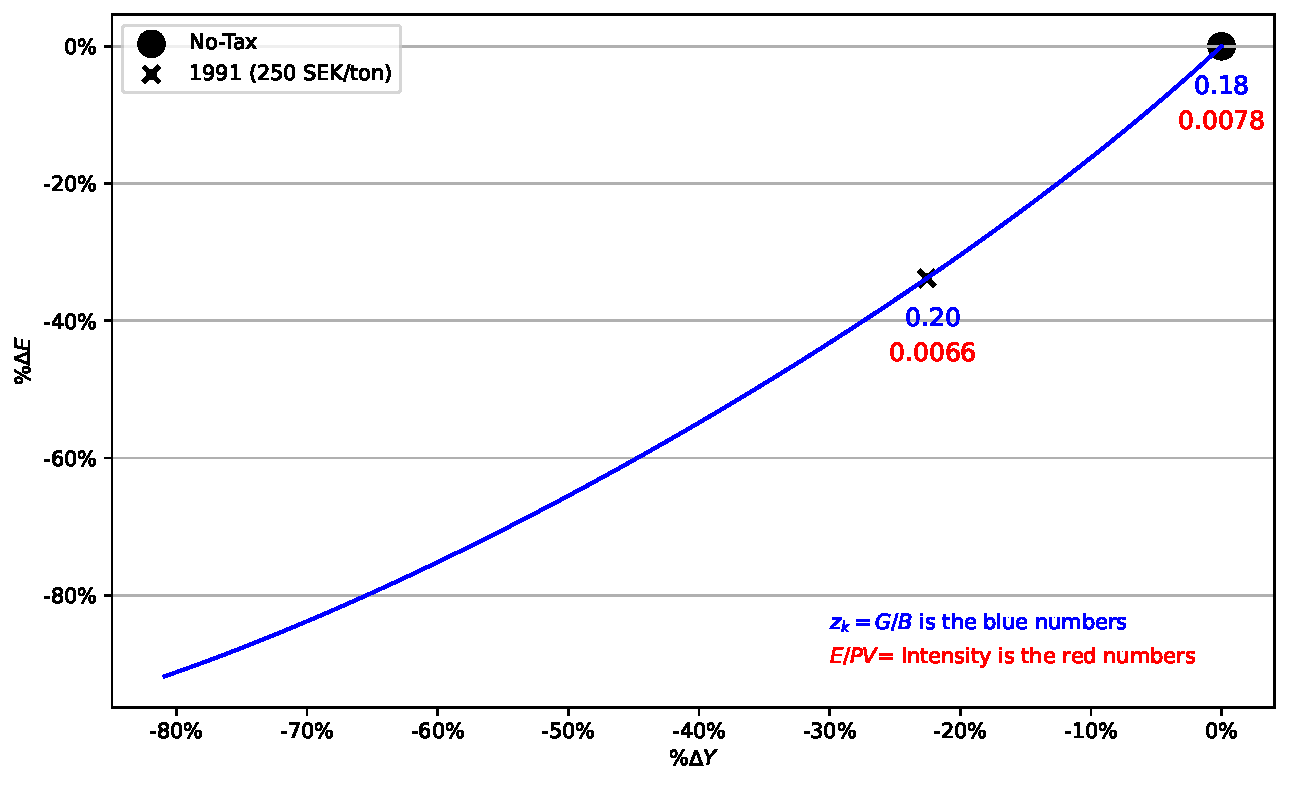
\includegraphics[width=.6\textwidth]{Figures/emission_production_2_2.pdf}}
		\only<4>{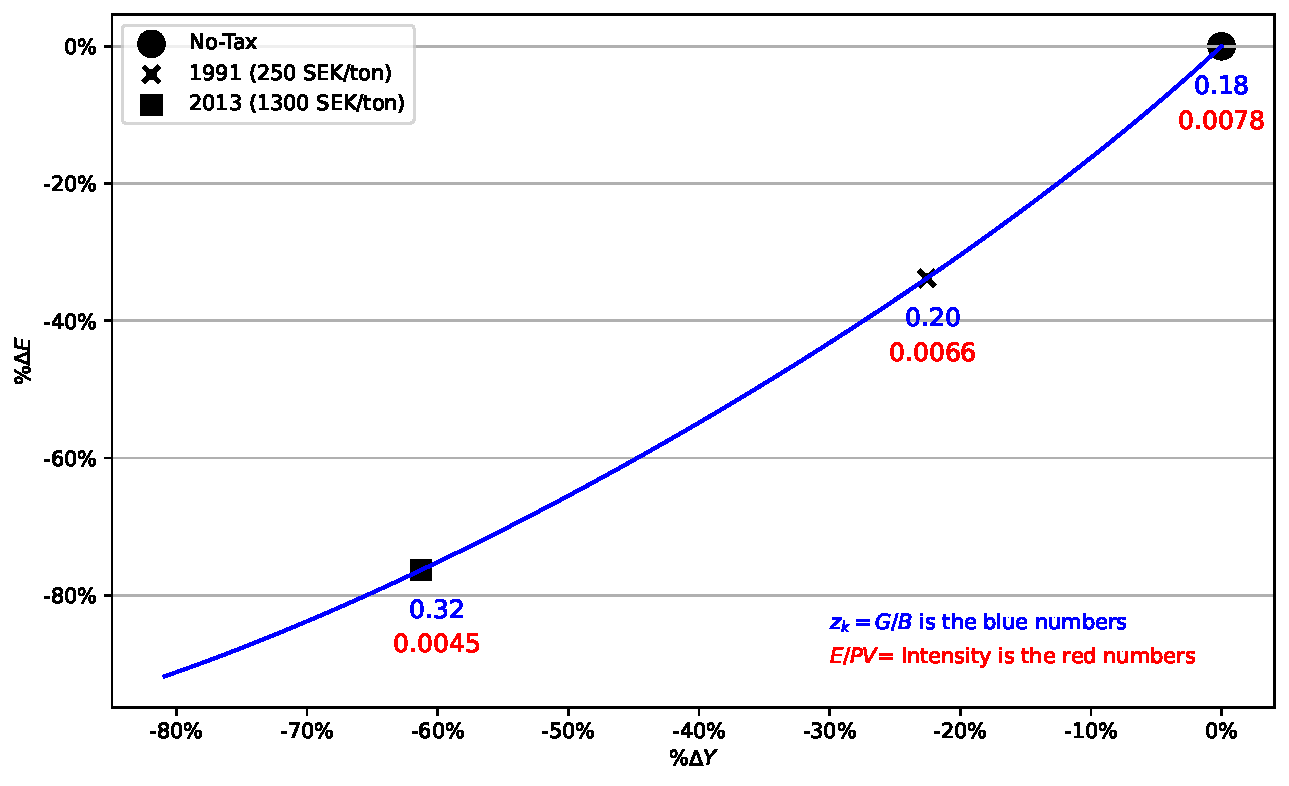
\includegraphics[width=.6\textwidth]{Figures/emission_production_2_3.pdf}}
		\only<5>{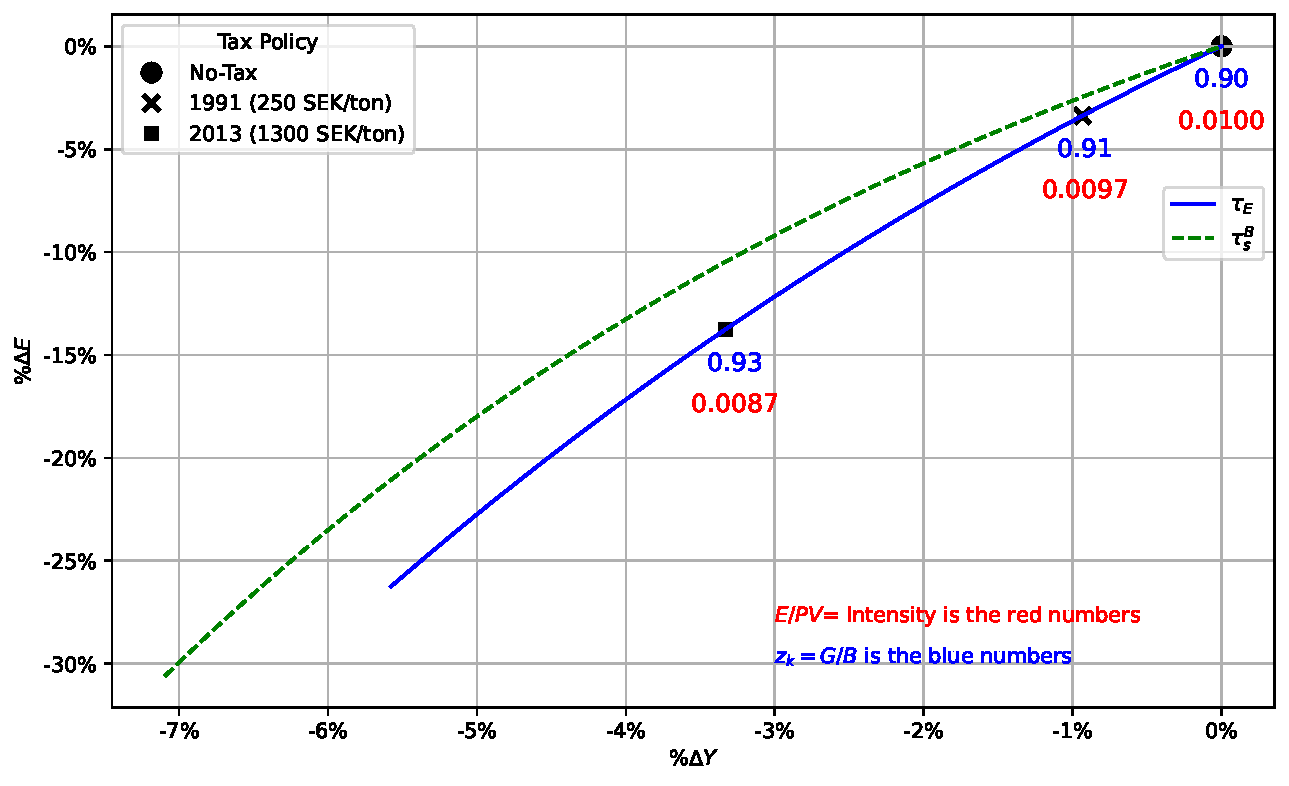
\includegraphics[width=.6\textwidth]{Figures/emission_production_3.pdf}}
		\only<6->{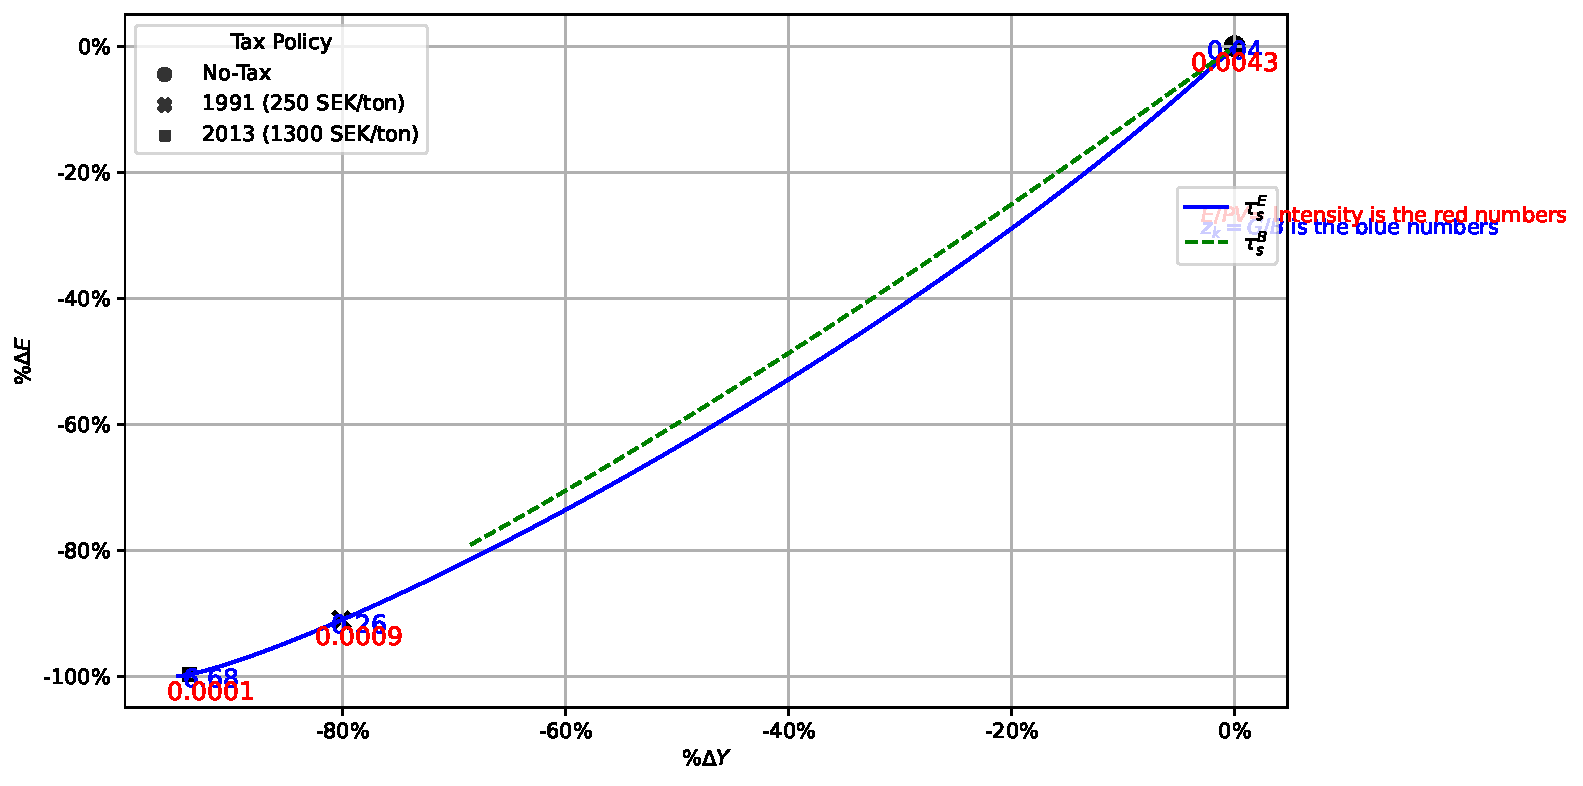
\includegraphics[width=.6\textwidth]{Figures/emission_production.pdf}}
	\end{figure}}
\end{frame}


\begin{frame}{Carbon Intensity and Tax}{{Counterfactual}}{
	\begin{columns}[t]
		\column{.7\textwidth}
		\begin{figure}[t]
		\centering
		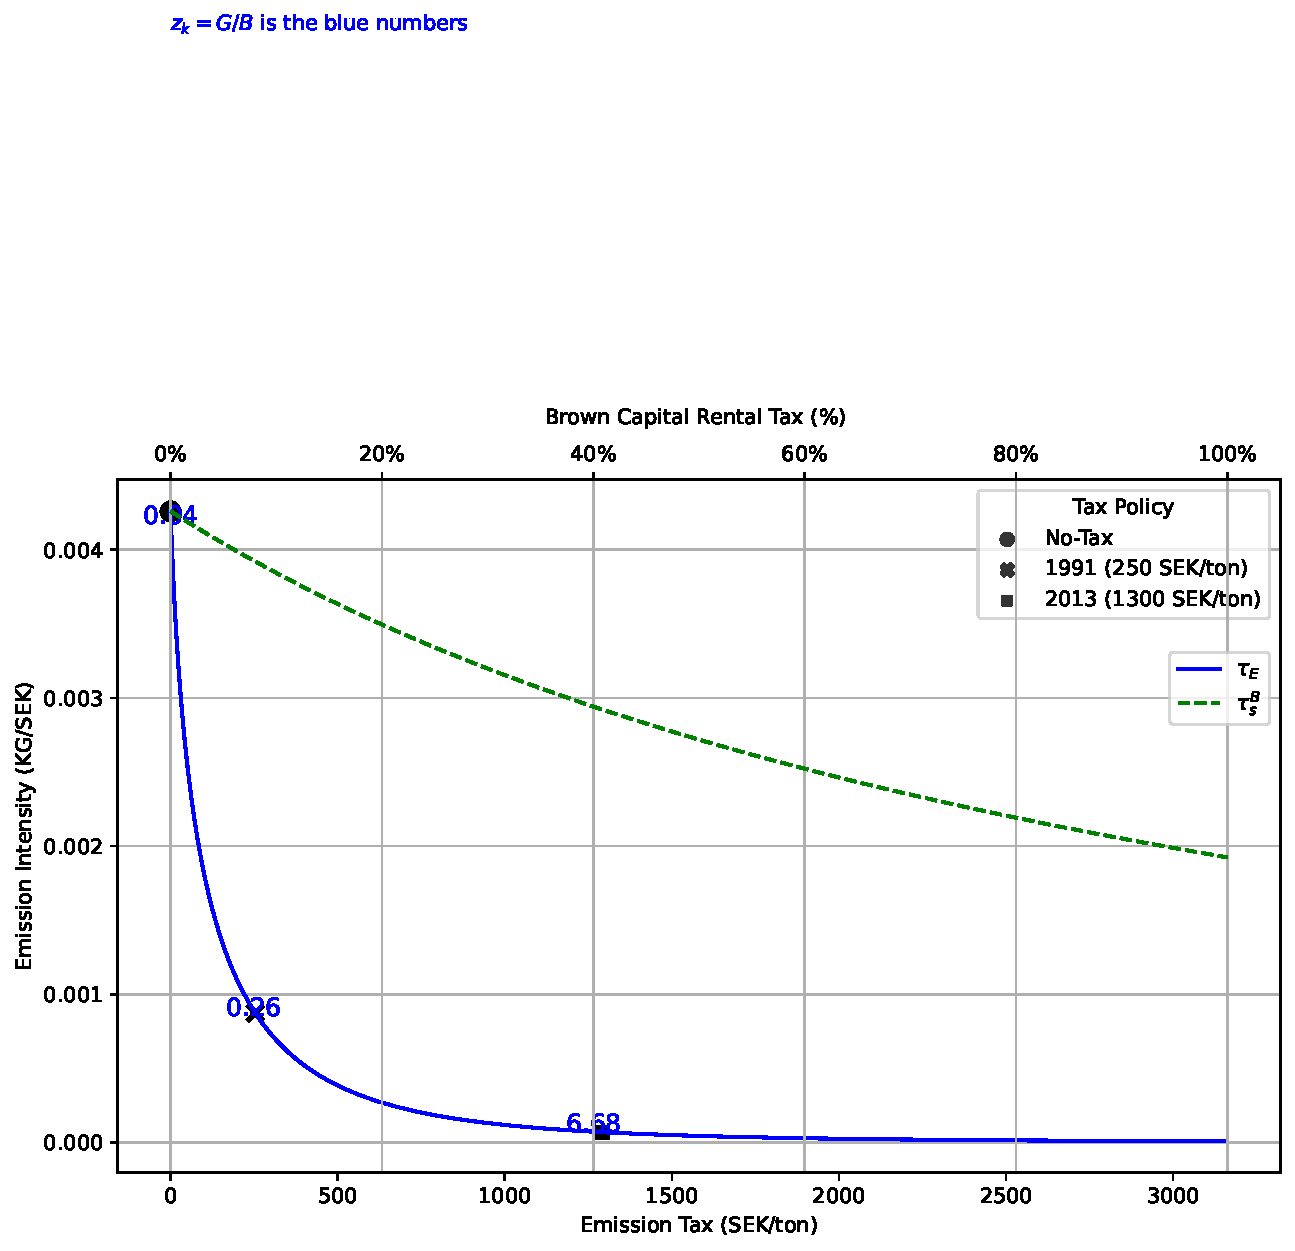
\includegraphics[width=.85\textwidth]{Figures/intensity_tax_premium.pdf}
		\end{figure}
		\column{.35\textwidth}
		\begin{table}[htbp]
			\begin{tabular}{ccc}
				\toprule
				$ \tau_E$ & $ \tau_G$ & $ \tau_B$ \\
				\midrule
					 100 &        9 \% &        2 \% \\
					 250 &       18 \% &        2 \% \\
					 500 &       27 \% &        4 \% \\
					1300 &       42 \% &       12 \% \\
					3000 &       55 \% &       26 \% \\
				\bottomrule
				\end{tabular}
		\end{table}
	\end{columns}
}
\end{frame}


\begin{frame}[noframenumbering]{Future Steps}
	\begin{enumerate}
		\item\textcolor<1->{fg!30}{ Develop Economic model with Emission }
		\begin{itemize}
			\item<1-| alert@1> Firms could R\&D
			\item<1-| alert@1> Add Household and Government
			\item<1-| alert@1> Firms could enter and exit the market
		\end{itemize} 
		\item\textcolor<1->{fg!30}{Characterize the allocation of resources }
		\item<1-| alert@1> {Provide a definition of Green and Brown capital}
		\item<1-| alert@1> Estimate the model by Swedish data 
		\item<1-| alert@1> Compare the optimal Policy with resource reallocation 
		\item<1-| alert@1> Discuss the cost of the environmental policies 
	\end{enumerate}
\end{frame}


\begin{frame}[noframenumbering]
	\begin{center}
		\Huge
		Thank you!
	\end{center}
\end{frame}

\appendix
\footnotesize
	\begin{frame}[allowframebreaks]{References}
			\bibliographystyle{aea}
\bibliography{literature}
		
	\end{frame}
	
	\normalsize

	\begin{frame}{Emission General Model}\label{Emission_General_Model}
		\begin{itemize}
			\item The firm's emission is:
			\begin{equation}
    \label{eq:firm_emission}
    E_{si} = \tilde{A}_{si}\tilde{K}_{si}^{\theta_s} L_{si}^{1-\theta_s} \quad,\qquad \tilde{K} = (
        \mu_s G_{si}^{\frac{\eta_s-1}{\eta_s}} + (1-\mu_s) B_{si}^{\frac{\eta_s-1}{\eta_s}}
    ) ^ {\frac{\eta_s}{\eta_s-1}}
\end{equation}
			\item The nominal profit for firms:
			\begin{equation}
				\pi_{si} = {(1+\tau_{si}^p) P_{si} Y_{si} - \left(\left[
        (1+ \tau_{G_{s}}) r_{si}G_{si} + (1+ \tau_{B_{s}}) r_{si}B_{si} + (1+ \tau_{l_{s}}) w_{si}l_{si}
    \right] + {\tau_{E} E_{si}}\right)}
			\end{equation}
			\end{itemize}
			\hfill
			\hyperlink{Production_Functions}{\beamerbutton{Back}}
	\end{frame}


	\begin{frame}{Firm's profit}\label{Firm_profit}
		\begin{itemize}
			\item The nominal profit for firms:
			\begin{equation}
				\pi_{si} = {(1+\textcolor{red}{\tau_{s}^p}) P_{si} Y_{si}} 
					\only<2->{- \left((1+\textcolor{red}{\tau_s^G}) \textcolor{blue}{r_{{s}}}G_{si}}
					\only<3->{+ (1+\textcolor{red}{\tau_s^B})\textcolor{blue}{r_{{s}}} B_{si}}
					\only<4->{+  (1+\textcolor{red}{\tau_s^W})\textcolor{blue}{w_{si}}l_{si}}
					\only<2->{\right)}
				\only<5->{- \textcolor{red}{\tau_{s}^E} E_{si}}
			\end{equation}
			\item where
			\begin{itemize}
				\item $\tau_{s}^p$ is the \textcolor{blue}{tax} / \textcolor{blue}{Demand preference} for the firm\\
				\item<2-> $\tau_{s}^G$ is the Green capital \textcolor{blue}{subsidy} / \textcolor{blue}{ESG preference} of Financier\\
				\item<3->$\tau_{s}^B$ is the Brown capital \textcolor{blue}{tax} / \textcolor{blue}{ESG preference} of Financier\\
				\item<4-> $\tau_{s}^W$ is the \textcolor{blue}{Labor market preference} to work in the green/brown sector {\tiny\citep{krueger2023sustainability}}
			\end{itemize}
	
			\item<6-> The firm chooses the optimal capital and labor to minimize the cost of production and then chooses the price level to maximize the profit
		\end{itemize}
		\hfill
		\hyperlink{Production_Functions}{\beamerbutton{Back}}
	\end{frame}
	
	\begin{frame}{Firm Decision}\label{Firm_solution}
		\begin{equation*}
			\max_{\textcolor{blue}{G_{si},B_{si},L_{si}}}  \quad
				- 		Cost \quad \text{s.t.} \quad \quad \hat{A}_{si}\hat{K}_{si}^{\beta_s} L_{si}^{1-\beta_s} = \bar{Y}_{si}
		\end{equation*}
	
		\begin{equation}
			\only<2->{\frac{G_{si}}{B_{si}} = \textcolor{blue}{z_{si}^k}} \uncover<3->{=  \left(
				\frac{\alpha_s}{1-\alpha_s} \frac{(1+\textcolor{red}{\tau_s^B})r_s + \textcolor{red}{\tau_s^E}\tilde{A}}{(1+\textcolor{red}{\tau_s^G})r_s}
			\right) ^{{\gamma_s}}}
		\end{equation}
	
		\begin{equation}
			\only<4->{\frac{L_{si}}{\hat{K}_{si}} = \textcolor{blue}{z_{si}^l}}
			\uncover<5->{ = \frac{1-\beta}{\beta}\frac{1}{\alpha_s}\left(
				\alpha_s + (1-\alpha_s) {\textcolor{blue}{z_{si}^k}}^{-\frac{\gamma_s-1}{\gamma_s}}
			\right)^{\frac{1}{1-\gamma_s}} \frac{(1+\textcolor{red}{\tau_s^G})r_s}{(1+\textcolor{red}{\tau_s^W})w_{si}}}
		\end{equation}
		\begin{equation}
			\only<6->{E_{si} = \frac{\tilde{A}_{si}}{\hat{A}_{si}}\left(
				\alpha_s {\textcolor{blue}{z_{si}^k}}^{\gamma_s - 1} + (1-\alpha_s)
			\right) ^ {\frac{\gamma_s}{1-\gamma_s}} {\textcolor{blue}{z_{si}^l}}^{1 - \beta} \bar{Y}_{si} }
			\uncover<7->{= \textcolor{blue}{\psi_{si}}\bar{Y}_{si}}
		\end{equation}
		\only<8->{	\begin{itemize}
			\item Firm will then charge markup over the marginal cost
		\end{itemize}}
	
		
		\hfill
		\hyperlink{Firm_solution_General}{\beamerbutton{General Model Solution}}
	\end{frame}


	\begin{frame}{Model}{Optimal Allocation}{\label{Firm_solution_General}}
		\begin{equation*}
			\max  \quad
				- 		Cost \quad \text{s.t.} \quad \quad \hat{A}_{si}\hat{K}_{si}^{\beta_s} L_{si}^{1-\beta_s} = \bar{Y}_{si}
		\end{equation*}
		\begin{equation*}
		z^k_{si} \equiv \frac{G_{si}}{B_{si}} = \left[
    \frac{\alpha_s}{1-\alpha_s} \dfrac{\frac{\partial }{\partial B}Cost_{si}}{\frac{\partial }{\partial G}Cost_{si}}
\right] ^ {\gamma_s} 
		\end{equation*}
		\begin{equation*}
			\begin{split}
    z^l_{si} \equiv \frac{L_{si}}{\hat{K}_{si}} & = \frac{1-\beta_s}{\beta_s} \frac{1}{1-\alpha_s} (\alpha_s {z^k_{si}}^{(\gamma_s -1)} + (1-\alpha_s))^{\frac{1}{1-\gamma_s}}\dfrac{\frac{\partial }{\partial B}Cost_{si}}{\frac{\partial }{\partial L}Cost_{si}}\\
    & = \frac{1-\beta_s}{\beta_s} \frac{1}{\alpha_s}(\alpha_s  + (1-\alpha_s){z^k_{si}}^{(1-\gamma_s )})^{\frac{1}{1-\gamma_s}}\dfrac{\frac{\partial }{\partial G}Cost_{si}}{\frac{\partial }{\partial L}Cost_{si}}
\end{split}
		\end{equation*}
		\hfill
		\begin{equation}
    E_{si} = {\frac{\tilde{A}_{si}}{\hat{A}_{si}}(\frac{\phi_{si}}{z^{l}_{si}})^{\theta_s} {z^{l}_{si}}^{\beta_s}} \bar{Y}_{si} = \psi_{si}\bar{Y}_{si}, \quad \text{where} \quad \phi_{si}  = \frac{(\mu_s  + (1-\mu_s){z^k_{si}}^{(1-\eta_s )})^ {\frac{\eta_s}{\eta_s-1}}}{(\alpha_s  + (1-\alpha_s){z^k_{si}}^{(1-\gamma_s )}) ^{\frac{\gamma_s}{\gamma_s-1}}} 
\end{equation}
		\hyperlink{Firm_solution}{\beamerbutton{Back}}
	\end{frame}
	\begin{frame}{Model}{Optimal firm level price}
		\begin{itemize}
			
			\item Now Firm need to choose the price level to maximize the profit:
			\begin{equation*}
    \max_{P_{si}} \quad \pi_{si} = P_{si}F_{si} - C_{si} {F}_{si}
\end{equation*}
			\item Firm-level real output is a function of the sector price, firm price, and sector real output (i.e. $F_{si} = (\frac{P_s}{ P_{si}})^{\sigma_s}{F}_s $)
			\item Therefore, because the optimal  ratio does not depend on the price, the ratio can be maximized out of the problem of the optimal determination of the price, leaving the firm’s real output as just a function of price
			\begin{equation}
    \begin{split}
         P_{si} =& \frac{1}{1+\tau_{si}^p}\frac{\sigma_s}{\sigma_s - 1} C_{si} \\
    \end{split}
\end{equation}
		\end{itemize}
	\end{frame}


\begin{frame}{Estimation / Calibration}\label{estimation_result}
	\begin{itemize}\footnotesize
		\item My goal is to estimate the parameters sector by sector for Sweden
		\item I just reasonably calibrate the model to match the summary statistics of \cite{martinsson2024effect}
		% \item I will set the $\hat{A} =$  \input{values/A hat estimate} to match the total output in the economy ($\sim 10$ BSEK).
	\end{itemize}
	\begin{table}[ht]
		\centering
		\label{your-label}
		\resizebox*{0.45\textwidth}{!}{\begin{tabular}{@{}ccc@{}}
		\toprule
		\textbf{Parameter} & \textbf{Value} & \textbf{Source/Moment} \\ \midrule
		\multicolumn{3}{c}{Panel A: Inputs} \\
		\midrule
		$\sigma$ & $\infty$ & Fully competitive \\
		$r$ & $5\%$ & - \\
		$w$ & $500$ TSEK & - \\
		$L$ & $250$ (sd = $900$) & \cite{martinsson2024effect}  \\
		\midrule 
		\multicolumn{3}{c}{Panel B: Calibrated Value} \\
		\midrule
		$\beta_s$ & $0.6$ &  \cite{martinsson2024effect}\\
		$\alpha_s$ & \input{values/alpha estimate} & \textcolor{red}{$G/B$}, \cite{wiedemann2023green} \\
		% $\gamma$ & \input{values/gamma estimate} & \cite{martinsson2024effect} \\
		% $\tilde{A}$ & \input{values/A tilde estimate} & $ E/PY $\\
		\midrule 
		\multicolumn{3}{c}{Panel C: Estimated Value} \\
		\midrule
		% $\beta$ & $0.6$ &  \cite{martinsson2024effect}\\
		% $\alpha$ & \input{values/alpha estimate} & \textcolor{red}{$G/B$}, \cite{wiedemann2023green}\\
		$\gamma$ & \input{values/gamma estimate} & $\Delta(\frac{E}{PY})/\Delta(\frac{C}{PY})$ \\
		$\tilde{A}$ & \input{values/A tilde estimate} & $ E/PY $\\
		\bottomrule
		\end{tabular}}
	\end{table}
		
		{
			\vfill
		\hyperlink{sensitivity}{\beamerbutton{Sensitivity of $\alpha$}}
		\hyperlink{results}{\beamerbutton{Back}}}
\end{frame}

\begin{frame}{Sensitivity analysis}\label{sensitivity}
	\begin{figure}[http]
		\centering
		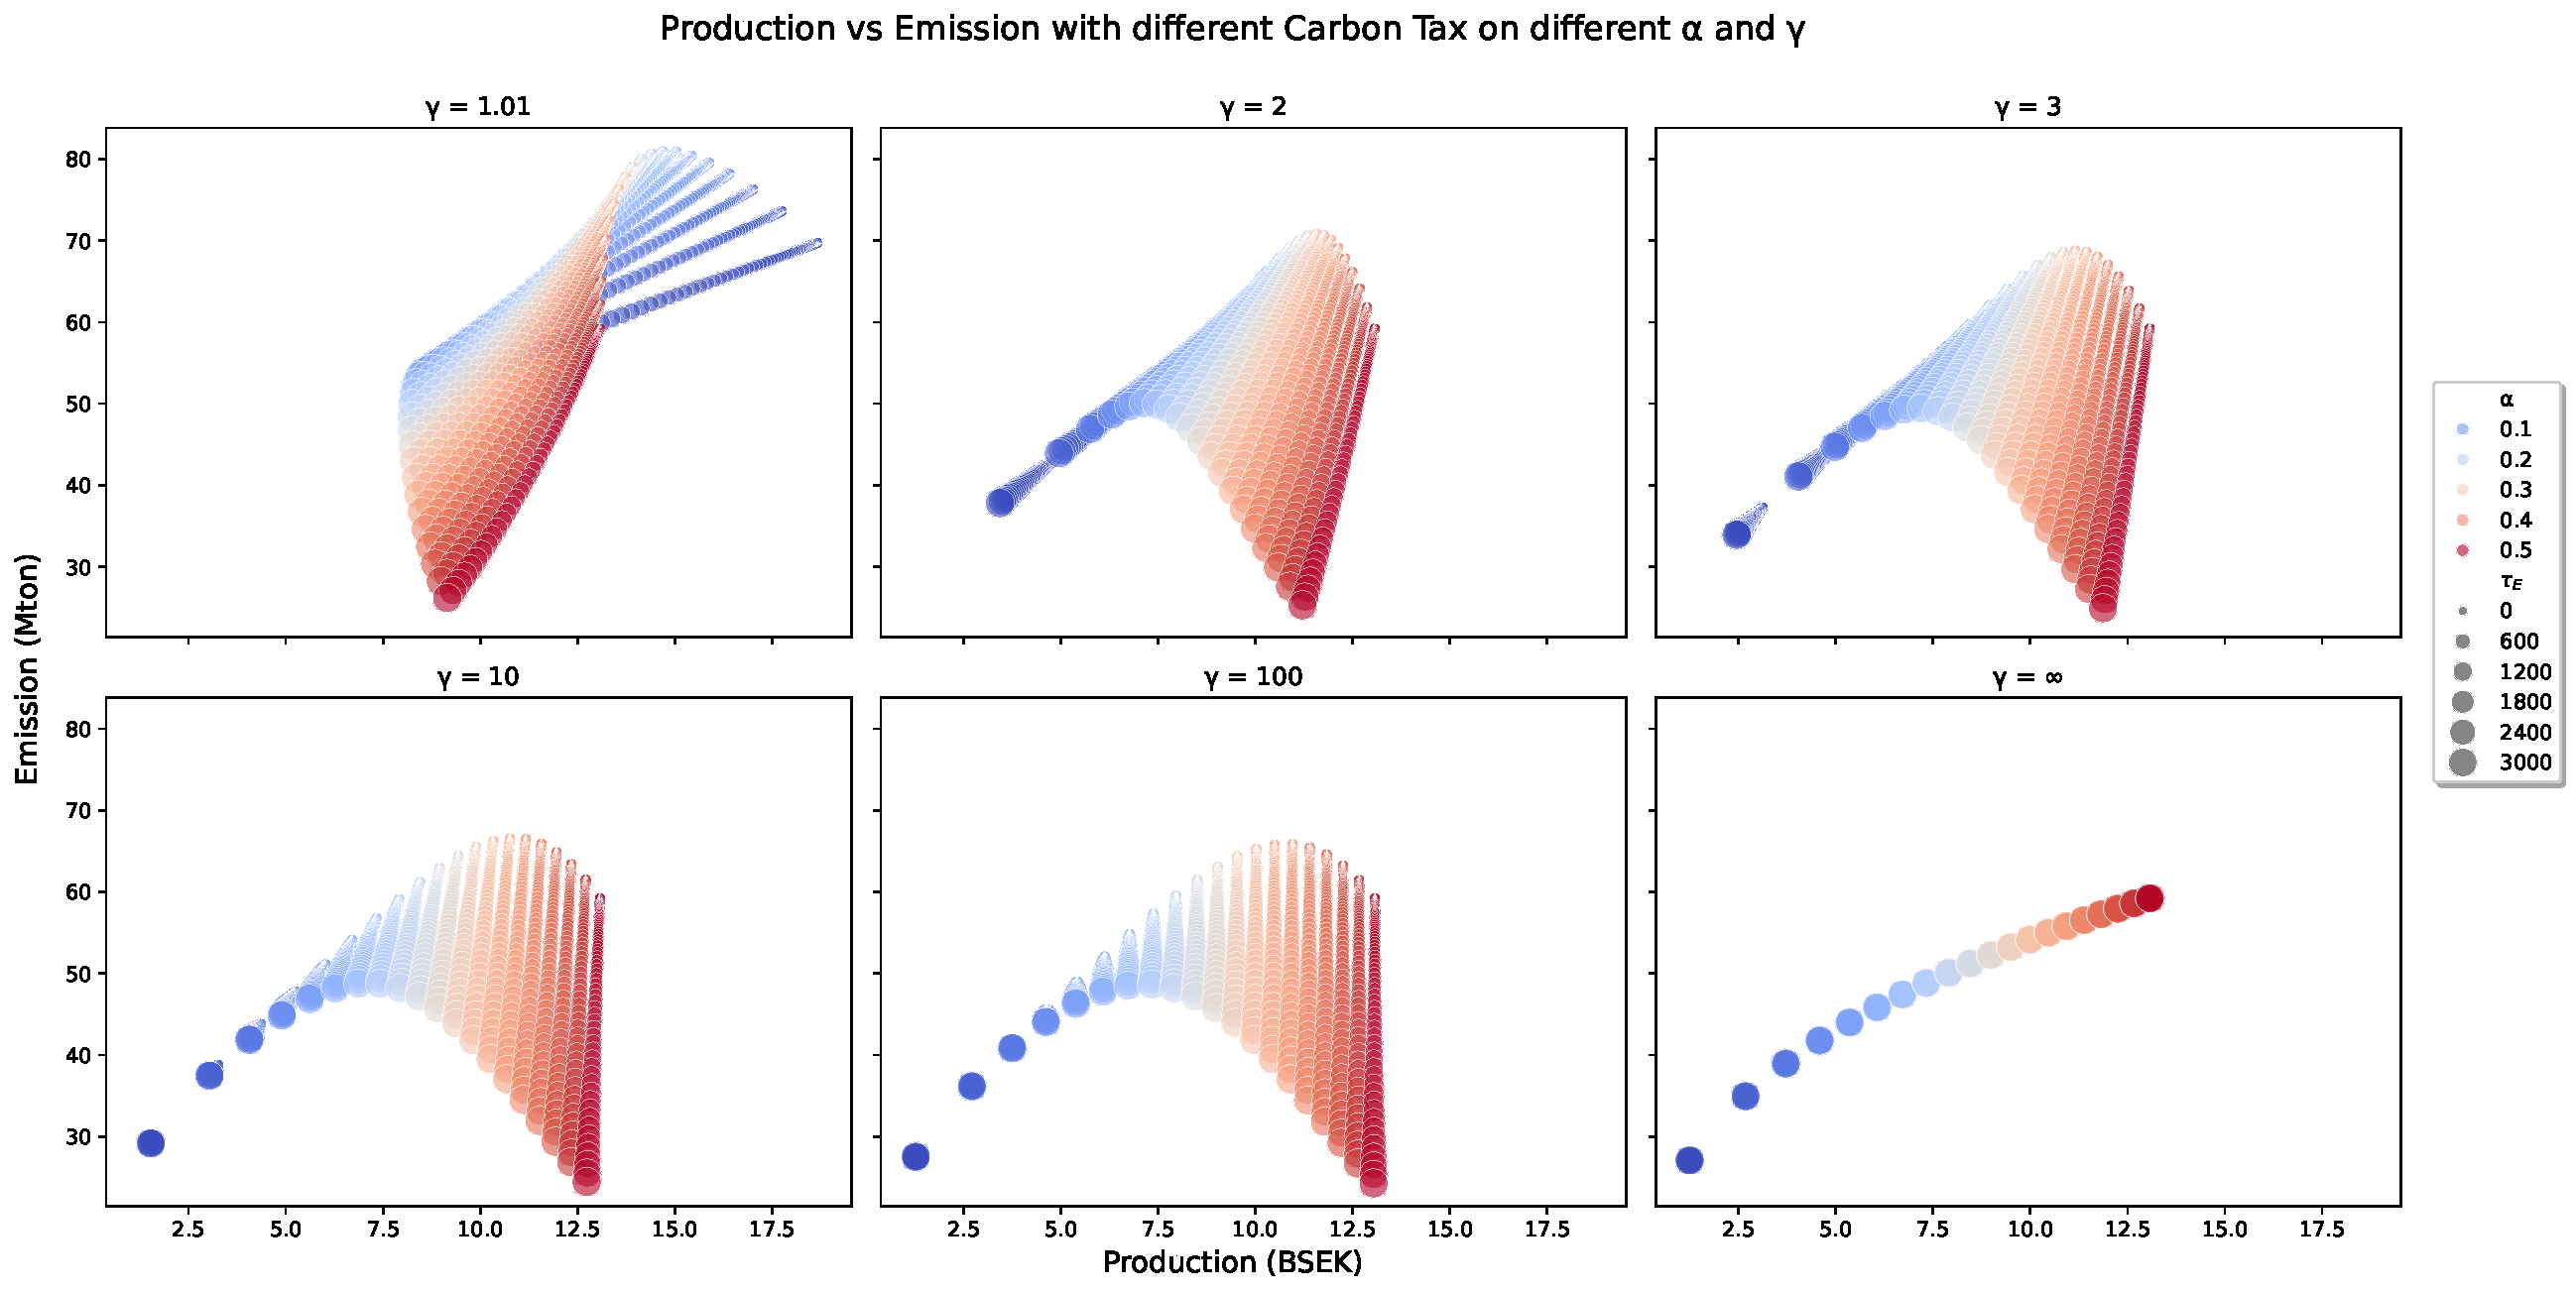
\includegraphics[width=0.9\textwidth]{Figures/production_emission.pdf}
	\end{figure}
	\hfill
	\hyperlink{estimation_result}{\beamerbutton{Back}}
\end{frame}

\begin{frame}{Carbon Intensity and Tax}{{Counterfactual}}{
	\begin{columns}[t]
		\column{.7\textwidth}
		\begin{figure}[t]
			\centering
		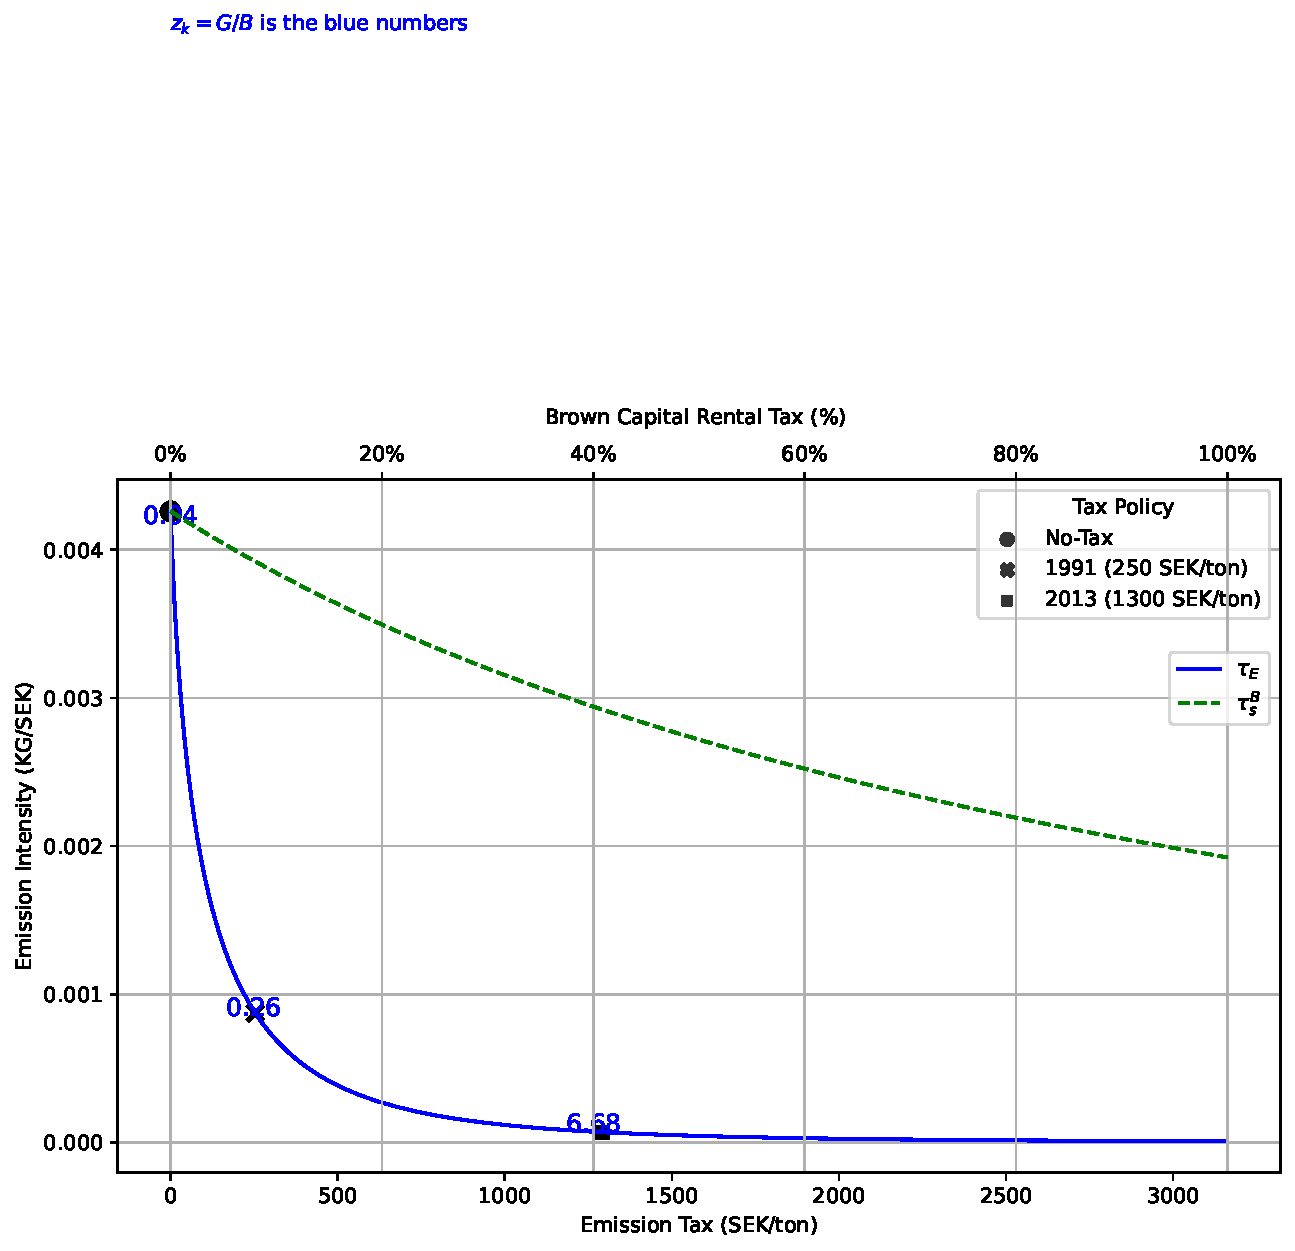
\includegraphics[width=.85\textwidth]{Figures/intensity_tax_premium.pdf}
		\end{figure}
		\column{.35\textwidth}
		\begin{table}[t]
			{\begin{tabular}{ccc}
\toprule
$ \tau_E$ & $ \tau_G$ & $ \tau_B$ \\
\midrule
     100 &        9 \% &        2 \% \\
     250 &       18 \% &        2 \% \\
     500 &       27 \% &        4 \% \\
    1300 &       42 \% &       12 \% \\
    3000 &       55 \% &       26 \% \\
\bottomrule
\end{tabular}
}
		\end{table}
	\end{columns}
}


\hfill
{\hyperlink{emission_production}{\beamerbutton{Emission and Production}}}
\end{frame}

\begin{frame}{Reallocation}{Resources allocation}\label{optimal_allocation}
\begin{itemize}
	\item Now, we need to find the optimal allocation of resources in the economy under two scenarios:
	\begin{columns}[T] % T aligns the columns from the top

		\uncover<2->{\begin{column}{0.5\textwidth} % First column
			\begin{gather} \label{eq:output_allocation_allocation}
    \hat{L}_{si} = \dfrac{\hat{A}_{si}^{\sigma -1}}{\sum_j \hat{A}_{sj}^{\sigma -1}}L_s\\ 
    \hat{G}_{si} = \dfrac{\hat{A}_{si}^{\sigma -1}}{\sum_j \hat{A}_{sj}^{\sigma -1}}\dfrac{z_s^k}{1 + z_s^k} K_s\\ 
    \hat{B}_{si} = \dfrac{\hat{A}_{si}^{\sigma -1}}{\sum_j \hat{A}_{sj}^{\sigma -1}}\dfrac{1}{1 + z_s^k} K_s
\end{gather}
		\end{column}}
		\begin{column}{0.5\textwidth} % Second column
			\begin{gather} \label{eq:emission_allocation}
				\uncover<3->{\tilde{L}_{si} = \dfrac{{\hat{A}_{si}^{\sigma -1}}/{\textcolor{red}{\tilde{A}_{si}^{\sigma}}}}{\sum_j \hat{A}_{sj}^{\sigma -1}/ \textcolor{red}{\tilde{A}_{sj}^{\sigma}}}L_s\\}
				\uncover<4->{\hat{G}_{si} = \dfrac{\hat{A}_{si}^{\sigma -1}/\textcolor{red}{\tilde{A}_{si}^{\sigma}}}{\sum_j \hat{A}_{sj}^{\sigma -1}/\textcolor{red}{\tilde{A}_{sj}^{\sigma}}}\dfrac{z_s^k}{1 + z_s^k} K_s\\ 
				\hat{B}_{si} = \dfrac{\hat{A}_{si}^{\sigma -1}/\textcolor{red}{\tilde{A}_{si}^{\sigma}}}{\sum_j \hat{A}_{sj}^{\sigma -1}/\textcolor{red}{\tilde{A}_{sj}^{\sigma}}}\dfrac{1}{1 + z_s^k} K_s}
			\end{gather}
		\end{column}
	\end{columns}			
\end{itemize}
\hfill
\hyperlink{planner_problem}{\beamerbutton{Back}}
\end{frame}



\end{document}


